\documentclass[nth=33]{humantech}

\usepackage{blindtext}
\usepackage{ragged2e}

\begin{document}
\title{Fast Photometric and Geometric Convergence in 3DGS SLAM}
\twocolumn[
\begin{@twocolumnfalse}
\begin{flushleft}
\maketitle
\begin{abstract}
\justifying
3D Gaussian Splatting (3DGS) enables photorealistic rendering, but its dense optimization restricts it to offline use. For robotics and wearable augmented reality, \emph{online mapping} is strictly demanded. Since "real-time" performance fluctuates with hardware, the true objective is achieving \emph{fast photometric and geometric convergence} under a bounded mapping budget. Two bottlenecks hinder this: tracking-oriented view selection dilutes updates, and shape-radiance ambiguity leaves spurious floaters in free space. To address these, we couple view-set expansion to completed updates and introduce Entropy-Regularized Count Balancing (ERCB) for equitable refinement. Geometrically, we bypass unstable positional gradients by directly suppressing spurious opacity via a causal Carve loss. By treating real-time operation as a strict constraint rather than a substitute for map quality, our formulation forces each optimization unit to immediately produce reliable geometry and appearance.
\end{abstract}
\vspace{20pt}
\end{flushleft}
\end{@twocolumnfalse}
]
\thispagestyle{firstpage}

\section{Introduction}
\label{sec:intro}

3D Gaussian Splatting (3DGS) has revolutionized photorealistic view synthesis~\cite{kerbl20233dgs}, but its computationally intensive optimization typically requires offline training. \emph{However}, autonomous agents and wearable augmented-reality systems strictly demand \emph{online mapping} to refine environments on the fly. While recent SLAM systems process streams quickly~\cite{matsuki2024monogs, huang2024photoslam}, "real-time" operation is an inherently ambiguous, hardware-dependent metric. Therefore, rather than engineering a system merely to meet an arbitrary frame rate, the fundamental objective \emph{must} be achieving \emph{fast photometric and geometric convergence}—maximizing map reliability under a bounded computational budget.

Fast convergence is hindered by two critical bottlenecks. First, uniform view sampling dilutes available updates across frames. We resolve this by coupling training-set growth to actual optimization progress and introducing Entropy-Regularized Count Balancing (ERCB) to correct training deficits~\cite{cartgs}. Second, due to shape-radiance ambiguity, misplaced Gaussians effortlessly replicate target colors by forming semi-transparent floaters in empty space~\cite{stablegs, wang2025efags}. Attempting to resolve this by simply translating Gaussians exposes a fundamental flaw: strict depth-sorting in the rasterizer causes abrupt gradient discontinuities when the rendering order changes. Therefore, rather than relying on unstable positional updates, we enforce a causal free-space Carve loss that directly suppresses opacity where depth evidence dictates empty space, effectively forcing geometric clustering~\cite{pagas2026, yu2024gof}.

Our contributions are summarized as follows:
\begin{itemize}
    \item We formulate an online 3DGS mapping framework optimized strictly for \emph{fast photometric and geometric convergence} under limited compute.
    \item We introduce Optimization-Guided View Growth and ERCB to correct severe optimization imbalances.
    \item We design an opacity-directed causal Carve loss to rapidly eliminate free-space artifacts, bypassing positional gradient discontinuities.
\end{itemize}

\section{Efficient Real-Time Online Gaussian Mapping}
\label{sec:method}

Our framework incrementally builds a Gaussian map from streaming RGB images and IMU measurements.
A DROID-SLAM-based frontend~\cite{teed2021droid} estimates camera poses and depths to initialize the Gaussian map and extend it to newly observed regions.
View Growth determines which images enter training, View Sampling selects images for each update, and Carve adds depth-based geometric supervision to map optimization.
% Declare the full-width overview at the end of the Introduction to target
% the top of the next page. Confirm final placement in the compiled paper.
\begin{figure*}[t]
  \centering
  % Prefer a manuscript-local copy when exporting this project to Overleaf.
  \IfFileExists{figure/overview.pdf}{%
    
\includegraphics[width=\textwidth]{figure/overview.pdf}%
  }{%
    \IfFileExists{../sections/02_method/figures/production/current/overview.pdf}{%
      
\includegraphics[width=\textwidth]{../sections/02_method/figures/production/current/overview.pdf}%
    }{%
      \fbox{\parbox[c][5cm][c]{0.95\textwidth}{\centering
        Draft: overview figure pending}}%
    }%
  }
  \caption{Overview of the proposed online Gaussian mapping framework.
  (a) View Growth expands the training set according to completed updates.
  (b) View Sampling allocates updates using cumulative selection counts.
  (c) Carve uses available depth evidence to suppress free-space opacity.
  View-management and ray diagrams are schematic; the shared map is a
  cutaway visualization of a map trained without Carve.}
  \label{fig:overview}
\end{figure*}

\noindent\textbf{Optimization-Guided View Growth.}
Frames between tracking keyframes provide additional viewpoints and appearance information.
Including more frames also spreads a limited number of updates across more images.
We therefore grow the training set according to completed mapping updates (Fig.~\ref{fig:overview}(a)).
Every $\kappa$ completed updates allow one additional image from the available observations to enter training; previously admitted images remain available for revisiting.
This ties view growth to actual optimization progress without requiring the remaining sequence length in advance.

\noindent\textbf{Entropy-Regularized View Sampling.}
Images admitted earlier have more opportunities to be selected for training.
To give less frequently selected images more updates while retaining randomness, we choose selection probabilities by minimizing
\begin{equation}
  \min_{\mathbf p\in\Delta}
  \sum_i p_i\Delta_i\Phi-\tau H(\mathbf p).
  \label{eq:view_sampling}
\end{equation}
Here, $p_i$ is the probability of selecting image $i$, and $\Delta$ contains
nonnegative probability vectors that sum to one.
We define $\Phi=\operatorname{Var}(\mathbf n)/(2\bar n)$ from cumulative
selection counts $\mathbf n$ with mean $\bar n$; $\Delta_i\Phi$ is its change
after selecting image $i$ once more.
The first term favors less frequently selected images.
The entropy term, $H(\mathbf p)=-\sum_i p_i\log p_i$, discourages concentration
on a few images, with $\tau>0$ controlling its strength.
Using these probabilities, we sample $K$ distinct images without replacement
and use each once over the next $K$ updates (Fig.~\ref{fig:overview}(b)).
% At zero total selections, use the symmetric/uniform initialization;
% the count-dispersion definition above applies once the mean is positive.

\noindent\textbf{Causal Free-Space Carve Loss.}
A map can reproduce image colors while retaining Gaussians in front of
observed surfaces, producing floating artifacts.
Depth observations provide evidence of free space between the camera and a surface.
Carve uses depths available at the current time, accounting for uncertainty
and a margin around the surface, to penalize opacity in this free space
(Fig.~\ref{fig:overview}(c)).
It adds an opacity gradient to the existing mapping objective without
directly updating Gaussian positions or shapes.

\noindent\textbf{Evaluation.}
We evaluate on the public RGB--IMU benchmarks RPNG~\cite{rpng_dataset}
and UTMM~\cite{utmm_dataset}, and on data we collected with Meta's Aria glasses.
Under a matched rendering budget, mean held-out PSNR exceeds that of
the reference method~\cite{vigsslam} by
1.60, 0.52, and 2.45\,dB, respectively.
Figure~\ref{fig:rgb_comparison} shows a selected held-out example in which
our system more faithfully reproduces the poster's logo and printed patterns.
This example illustrates our goal of turning incoming observations into
faithful appearance reconstruction within a limited mapping budget.
Figure~\ref{fig:carve_comparison} is reserved for the Carve geometry ablation.
% Source: paper/latex/sec/5_results.tex, tab:rendering_comparison.
% These are fixed-work mapping quality results, not measured real-time FPS.
% F04 provenance: exp94, 34,437 physical mapping renders per method,
% same evaluation pose, Carve off. Selected high-gain frame, not a mean.
% Record the configuration in the final experimental setup; this image
% does not isolate individual components or establish time-to-quality.

\begin{figure}[t]
  \centering
  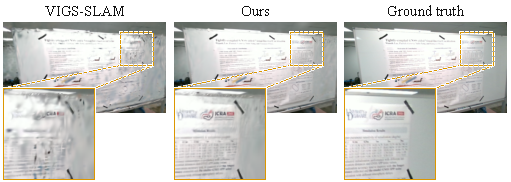
\includegraphics[width=\linewidth]{figure/rgb_comparison.pdf}
  \caption{Held-out rendering comparison between VIGS-SLAM~\cite{vigsslam}
  and our method on RPNG \texttt{table\_06} under a matched rendering budget.}
  \label{fig:rgb_comparison}
\end{figure}

\begin{figure}[t]
  \centering
  \IfFileExists{figure/carve_comparison.pdf}{%
    \includegraphics[width=\linewidth]{figure/carve_comparison.pdf}%
  }{%
    \fbox{\parbox[c][2.6cm][c]{0.92\linewidth}{\centering
      Draft: solid-ellipsoid comparison pending\\
      Without Carve / With Carve}}%
  }
  \caption{Planned Carve ablation using solid ellipsoids from the same
  viewpoint and identical opacity-display and scale settings.
  Draft: models, region-GT metrics, and held-out PSNR remain to be supplied.}
  \label{fig:carve_comparison}
\end{figure}


\section{Conclusion}
We present an online Gaussian mapping system for efficient optimization of
appearance and geometry, and report an average held-out PSNR gain of
1.25\,dB over the reference method across 17 scenes under matched rendering budgets.
Our system introduces optimization-guided view management to control view
admission and update allocation, and a causal Carve loss to suppress spurious
opacity in free space using depth observations.
This approach provides a foundation for real-time online mapping in robots
and wearable augmented-reality systems that need reliable maps of their
surroundings during operation, with limited computation and without waiting
for offline refinement.


\small{
\bibliographystyle{abbrv}
\bibliography{bibliography}
}
\end{document}
